\documentclass{llncs}
%\usepackage[cp1250]{inputenc}
\usepackage[utf8]{inputenc}
%\usepackage[czech]{babel}
\usepackage{graphicx}
\usepackage{tipa}


\begin{document}
\newtheorem{Definition}{Definition}
\title{Making Community and ASR Join Forces in Web Environment}

\author{Old\v{r}ich Krůza and Nino Peterek}
\institute{Charles University in Prague\\
           Faculty of Mathematics and Physics\\
           Institute of Formal and Applied Linguistics\\
           Malostranské nám. 25, Prague, Czech Republic\\
           kruza@ufal.mff.cuni.cz, peterek@ufal.mff.cuni.cz}

\maketitle

\begin{abstract}

The paper presents a system for combining human transcriptions with automated
speech recognition to create a quality transcription of a large corpus in good
time. The system uses the web as interface for playing back audio, displaying
the automatically-acquired transcription synchronously, and enabling the visitor
to correct errors in the transcription. The human-submitted corrections are then
used in the statistical ASR to improve the acoustic as well as language model
and re-generate the bulk of transcription. The system is currently under
development.\\
The paper presents the system design, the corpus processed as well as
considerations for using the system in other settings.

\end{abstract}

\section{Introduction}

For a setting where recorded speech data are available, it is often desirable to
obtain a transcribed version of the spoken words because processing digital text
is much simpler than processing digital audio. Human transcription is costly and
no automatically acquired transcription is perfect, so human revision of ASR
output is a common scenario.

In our setting, where an uncatalogized spoken corpus and a community of lay
volunteers are available, we feel a need for a system that would employ the
modern speech-recognition technology and thoroughly exploit the precious brain
cycles of the involved humans. The web with its ever-growing possibilities
offers a neat platform for creating such a system.

\subsection{Spoken corpus of Karel Mako\v{n}}

Karel Mako\v{n} (1912-1993) was a Czech mystic who authored 27 books on
spirituality and Christian symbolism, and translated and commented 28
others\footnote{http://www.makon.cz/}.
Aside from his writing, he was giving talks in a close, private circle of
friends as the topics he was covering were not safe to express openly under the
socialist regime. His friends and apprentices recorded most of his lectures on
magnetic tapes. The recording started in late 60's using reels, then switched to
cassettes in the course of the 70's and went on until Mako\v{n}
ceased to give lectures in 1992, one year before his death.

The recordings were archived in the homes of their makers, losing the quality
as the magnetic signal was slowly fading over time. Attempts have been made to
digitize the material, but using little to no automation only a
fraction has been converted, leaving the rest of the material at time's mercy. A
systematic digitization took place only from 2010 to 2012 when most of the material
was converted to wav files.

The complete corpus, as of the time of writing, comprises about 1000 hours and
is available on-line\footnote{http://www.makon.fm/}. Our work deals
with processing this corpus, although the system under development is intended to
work on any data and we hope it will be useful in a broader spectrum of
settings.

\section{Motivation for transcription}

The digitized corpus is largely unstructured. The only metadata we have, are
years and sequential numbers in case of the cassettes. For some reels, there are
handmade indexes listing the topics covered and the corresponding time positions on the
counter of the device. These are typed on paper and have been photographed. The
indexes, however, cover only 76 of the 1096 total files.

This is a similar setting to the Malach\cite{malach} project. Malach was
approached by doing automatic speech recognition and building a search engine on
the ASR output. Our setting differs from that of Malach significantly, as we
merely have to deal with material by one single speaker, and we just have to handle about one thousand hours
in comparison with Malach's stunning one hundred sixteen thousand hours. This
plus the fact that there is an active community around the legacy of Karel
Mako\v{n} motivates us to attempt a full, high-quality, verbatim transcription
of Mako\v{n}'s talks.

\section{Architecture of the system}

Obviously, there are two basic ways to do speech-to-text transcription:
\begin{itemize}
\item{manually,}
\item{automatically.}
\end{itemize}
Manual transcription usually delivers very high quality, but it is unbearably
time-consuming. Automatic transcription can be quite fast, but the amount of
errors leaves much to be desired. Hence, we propose and are developing a system
to draw on the power of both to converge quickly to a good transcription.

\begin{figure}[htpb]
\includegraphics[scale=0.6]{arch.eps}
\caption{Schema of the system architecture}
\label{fig:arch}
\end{figure}

Figure~\ref{fig:arch} outlines the system architecture:
\begin{enumerate}
\item{An initial transcription is obtained by means of an automatic speech recognition
system.\label{enum:arch:init}}
\item{The resulting transcription is transformed into a JavaScript data
structure suitable for synchronous displaying on the web
interface.\label{enum:arch:htk2sub}}
\item{Visitors use the web interface to listen to the recordings,
at the same time seeing the synchronized transcription.}
\item{When encountering an error in the transcription, the visitor selects the
erroneous text and edits it, entering the correct transcription.}
\item{The corrected subtitle is immediately saved, so that it is shown on
subsequent requests of that passage.}
\item{The corrected subtitle is added to the training data of the ASR system.}
\item{The ASR model is re-trained with the new training data.}
\item{The re-trained ASR model is applied and the bulk of the transcription that
has not yet been human-corrected, is re-generated.}
\end{enumerate}

\subsection{First transcription}

We did some first experiments to obtain the initial transcription. We tried
to train an acoustic model on 15 minutes of manually transcribed material from
one of the recordings. The training was executed using HTK\cite{htk}. We also
adapted the acoustic model from CUCFN\cite{cucfn} to Makoň's speech using the
mentioned 15 minutes of manual transcription.

For language modeling, we trained a bigram model on Karel Makoň's books and one
on PDT\cite{pdt}. We're searching for a fitting ASR configuration to use the
models. The current results on ASR for Czech\cite{czasr} give us certain
expectations with respect to accuracy.

\subsection{Web interface}

The web interface where people can collaborate on speech transcription is a
cornerstone of the whole project. The audio is played back by browser's native
HTML5 \texttt{\textless{}audio\textgreater} element, falling back to
flash\footnote{http://www.adobe.com/products/flashplayer.html} where HTML5 is
not supported\footnote{jPlayer was used for this; http://jplayer.org/}. The
subtitles are shown as three lines of text with the current word being
highlighted. The lines scroll down as the recording is played back. This was
chosen for ergonomic reasons. Two other possible implementations that came into
mind were rejected:
\begin{enumerate}
\item{a horizontally-scrolling line of text, like a
\texttt{\textless{}marquee\textgreater} HTML element,\label{enum:subs:marquee}}
\item{subtitles like in a movie: one phrase shown at a time, which disappears
and is replaced by a new one.\label{enum:subs:srt}}
\end{enumerate}
Using a marquee-like solution (point \ref{enum:subs:marquee}) would cause
constant scrolling in a non-constant speed, since the rate of the speech varies.
This would quickly become annoying.

Using a movie-subtitle-like solution (point \ref{enum:subs:srt}) has the
disadvantage of making it impossible to select (and thus correct) a span of
text reaching across the given phrases.

In our solution, several lines are shown, they are horizontally static, and the
current word is highlighted, always being kept on the middle line (unless the
beginning or end of the recording is being played back). This delivers the reader enough
context and feels similar to reading static text. A drawback of
this method is that showing many lines gets computationally intense. We wrap
each word into a dedicated HTML element to be able to keep track of the
currently played word and to be able to track down the corresponding subtitles
when the user selects and corrects some text chunk. A good trade-off seems to be using
three lines. There is always enough context, it is never hard to spot the
highlighted word, and the browser stays responsive.

The highlighting of the current word still has a small difficulty. Since the
time-update event, which triggers re-drawing of the highlighted word, is quite
coarsely granular -- i.e. it fires only about 4 times per second --, it happens that
a word is highlighted with a noticeable delay. This reduces the comfort slightly
but can be avoided using look-ahead methods.

As hinted at in point \ref{enum:arch:htk2sub} of the architecture outline, the
subtitles are stored in a JavaScript structure. To be more precise, we're
storing it in the JSONP\cite{jsonp} format.
This allows us to have the subtitles on an external
CDN\footnote{Content-delivery network} and dedicate the web server to processing
the corrections. Another obvious advantage is that the browser can parse the
subtitles rapidly, not losing responsivity for a long period.

\section{Dealing with submitted corrections}

Processing the submissions from the visitors is probably the most important point
of the work. Working collaboratively on large data over web is a very popular
approach, most notably exploited by
Wikipedia\footnote{http://www.wikipedia.org/}. Our setting shares some notions
with that of Wikipedia, but is obviously quite different. Not only because our
data are acoustic but mainly because in our case, there is one correct output
that we hope the users to provide, whereas in case of Wikipedia, the users are
creative. This makes our task much easier in respect of conflict resolution.
When two people edit the same Wikipedia article at the same time, an interactive
edit-conflict procedure has to be
employed\footnote{http://en.wikipedia.org/wiki/Help:Edit\_conflict}.

To explain our situation, we'll first outline what happens when a correction is
sent by a visitor.
\begin{enumerate}
\item{The visitor selects the subtitles where the error is contained. The
selection is automatically padded to whole words.}
\item{The selected subtitles are replaced by a textarea where the words are
copied.}
\item{When the textarea loses focus, and if it had changed, then the new text is
sent to the server using an
AJAX\cite{ajax} request. Along with the text, the timestamp of the first word
and of the one after the last word is sent.}
\item{On the server, the correction is saved into the database.}
\item{The corresponding audio sequence is extracted and matched against the
provided text.

If the forced alignment fails, the process ends
and no further modifications take place; an error response is sent to the
client.

If, on the other hand, the forced alignment of the provided subtitles to
the audio succeeds, then the individual words get timestamps
and the process continues.\label{enum:corr:align}}
\item{The corrected span of subtitles is replaced with the submitted aligned
text and the transcription is saved.}
\item{The submitted transcription is added to training data for the acoustic
model.}
\item{The submitted transcription is added to the training data for the language
model.}
\item{Re-training of the model is scheduled.\footnote{Actually re-training the
model and re-recognizing the whole corpus after every submissions is, of course,
infeasible.}}
\end{enumerate}

Notice that % 1) all submissions are saved into the database and 2)
if two people
send overlapping corrections, they are simply pasted onto each other. The
intersection is saved from the latter of the concurring submissions.
Assuming they were both correct, there is no conflict.

If we give up the assumption of the correctness of the submissions, we have two
ways of dealing with that. Firstly, notice point \ref{enum:corr:align} of the
correction sequence: If the alignment fails, then the subtitle is not saved.
This protects the system from outright vandalism and spam, since transcriptions
that are too far from the audio will be automatically rejected.

Other, more subtle forms of errors introduced by the visitors will naturally be
harder to compensate. One thing we might do, is to track which correction comes from
which user. If a user tends to consistently make a certain kind of mistake, it
may be possible to revert it, or to set up a group of proof-readers. This is
pure theory though. We'll have to deal with these problems when they come.

We were making a simplification up to this point: Upon submission of a corrected
subtitle, we cannot just add this to the training data. We also have to remove
previous corrections of the same passage, so that previously introduced errors
can be compensated.

\subsection{Foreign words}

Another scenario that brings in complications is, when foreign words or any
words with non-standard pronunciation are a part of the corrected subtitle.
Suppose that the name \emph{George} appears in the audio and is not correctly
recognized. Also suppose the name is not present in the dictionary of the speech
recognition system. Since the mechanism for accepting or rejecting a submission
is based on acoustic fit and we use a simple rule-based word-to-phonemes
converter\footnote{We use phonetic alphapet designed by Psutka et al. 1997
\cite{czphabc} based on Czech phonology as described by Palková 1992 \cite{czphon}},
if the user enters \emph{George}, the word-to-phonemes
converter will assume pronunciation \textipa{/gEorgE/} instead of the correct
\textipa{/dZO:\*rdZ/} -- and thus will likely be rejected as non-matching.

We approach the problem by instructing the users to type in foreign words in
their phonetic transcription. In this case, \emph{džordž}. After the subtitle is
saved, the words become data structures with independent word forms and
pronunciations. Then, the proper spelling \emph{George} can be introduced.

%\subsection{Selecting data to correct}
%
%One interesting aspect of our setting is that we can influence which part of the
%corpus will be subject to corrections. We can recommend to visitors, which parts
%they should listen to right now.
%
%With enough training data, the system reaches a state where more training data
%no longer increases the accuracy\cite{
%    % TODO: někoho citovat
%}. Therefore, it is good to choose such samples for manual transcription that
%will globally maximize the precision of the model in the point of training-data
%saturation. This set can be to a certain degree approximated\cite{
%    % TODO: citovat ty, co popisujou výběr vhodných trénovacích dat
%}. % TODO: popsat, jak se to přibližně dělá

\section{Using the system in other settings}

As much as our primary aim is to process this specific corpus, we hope the
functionality developed to be applicable in a wide range of settings. Applying
the system for a different corpus should be straight-forward. Complications
could arise if the corpus were stored in smaller files since we don't take care
of playing one file after another: we assume that they are separate and the user
is only ever interested in one specific file at a time.

Using the system for a corpus in another language would also make modifications
necessary. Mainly the word-to-phonemes conversion would have to be implemented
in a way that is suitable for the given language. Of course the whole ASR can be
replaced -- and we plan to do this to try out different ones.

One part that lends itself neatly for modifications and re-use is the web
interface. For data, where audio, or video for that matter, and aligned
transcription are available, the interface can be used as a generic subtitle
displayer.

In music, the audio-text synchronous display could be used for collaborative
transcription of lyrics or even for karaoke. One possible serious drawback in
this would be the difficult matching of lyrics to audio. The music mixed into
the words, artistic interpretation of the vocalist and a variety of speakers
(singers actually) would likely make the alignment much less robust. In a
setting though, where the aligned lyrics with potential errors are on input, the
system could still be well used to for display and gathering corrections.

In language teaching, students could use the system to match spoken words with
written ones to learn pronunciation of their language of interest. Introducing
deliberate errors and expecting corrections could be a way of examination.

\section{Conclusion}

The described system is under development. Much of the functionality
has already been implemented, although the current form of the user interface is
crude at best. Our work on this project has merely begun. We are thrilled to
develop a system that on one hand will systematize and make available maybe the
most comprehensive opus on Christian mystic in Czech, on the other hand will
open new possibilities in collaborative transcription of speech.

\section*{Acknowledgments}

The research was supported by SVV project number 265 314.\\
\\
This work has been using language resources stored
by the LINDAT-Clarin project of the Ministry of
Education of the Czech Republic (project LM2010013).

\bibliographystyle{splncs}

\begin{thebibliography}{}

\bibitem{malach}
W Byrne, D Doermann, M Franz, S Gustman, J Hajic, D Oard, M Picheny, J Psutka, B
Ramabhadran, D Soergel, T Ward, Wei-Jing Zhu
\emph{Automatic recognition of spontaneous speech for access to multilingual
oral history archives}
in Proc. Eurospeech 2003, Geneva, Switzerland
http://www.ee.umd.edu/~oard/pdf/tsap04.pdf

\bibitem{htk}
S Young, G Evermann, M Gales, T Hain, D Kershaw, X A Liu, G Moore, J Odell, D
Ollason, D Povey, V Valtchev, P Woodland
\emph{The HTK Book}
2006\\
http://htk.eng.cam.ac.uk/

\bibitem{cucfn}
W Byrne, J Hajič, P Ircing, F Jelinek, S Khudanpur, J McDonough, N Peterek
and J Psutka
\emph{Large Vocabulary Speech Recognition for Read and Broadcast Czech}
Lecture Notes in Computer Science; Springer Berlin / Heidelberg; 1999\\
http://www.springerlink.com/content/8f82hg9y13tylthc/fulltext.pdf

\bibitem{pdt}
A B\"{o}hmová, J Haji\v{c}, E Haji\v{c}ová, B Hladká
\emph{The Prague Dependency Treebank: A Three-Level Annotation Scenario}
2007\\
http://www.scientificcommons.org/43211198

\bibitem{czasr}
J Psutka, J Hajic, W Byrne
\emph{The development of ASR for Slavic languages in the MALACH project}
in Proc. ICASSP 2004\\
http://svr-www.eng.cam.ac.uk/~wjb31/ppubs/icassp04-malach-final.pdf

\bibitem{jsonp}
B Ippolito
\emph{Remote JSON - JSONP}
2005\\
http://bob.pythonmac.org/archives/2005/12/05/remote-json-jsonp/

\bibitem{ajax}
J J Garrett
\emph{Ajax: A new approach to web applications}
2005\\
http://mmccauley.net/com601/material/ajax\_garrett.pdf

\bibitem{czphabc}
J Nouza, J Psutka, J Uhlíř
\emph{Phonetic alphabet for speech recognition of Czech}
Radioengineering Vol.6, pp. 16-20, 1997\\
http://www.radioeng.cz/fulltexts/1997/97\_04\_04.pdf

\bibitem{czphon}
Z Palková
\emph{Fonetika a fonologie Češtiny}
Univerzita Karlova, Praha 1992

\end{thebibliography}
%\bibliography{paper}
\end{document}
